\documentclass{beamer}
\usepackage[T1]{fontenc}
\usepackage[utf8]{inputenc}
\usepackage{lmodern}
\usepackage[francais]{babel}
\usepackage{graphicx}
\usepackage{beamerthemeWarsaw}
\expandafter\def\expandafter\insertshorttitle\expandafter{\insertshorttitle\hfill\insertframenumber\,/\,\inserttotalframenumber}

\title{Des réseaux et des drones}
\author{Olivier \bsc{Boissard}, Kevin \bsc{Boulala}}
\institute{Université de Franche Comté}
\date{\today}

\begin{document}

\begin{frame}
  \titlepage
\end{frame}

\begin{frame}
	\tableofcontents[]
\end{frame}

\section{Les drones}
\subsection{Définition}
\begin{frame}
  \frametitle{Définition 1/2}
  \framesubtitle{C'est large quand même}
  \begin{block}{L'environnement}
    \begin{itemize}
      \item Terrestre (ex : Vitirover, Opportunity, Curiosity)
      \item Marin (ex : Protei par César Harada)
      \item Spatial (ex : X-37B de Boeing)
      \item \textbf{Aérien} (ex : Quad DJI INSPIRE X5 PRO de Flying Eye)
    \end{itemize}
  \end{block}
  \begin{columns}
    \begin{column}{.25\textwidth}
      \includegraphics[width=\textwidth]{../Images/Curiosity.jpg}
    \end{column}
    \begin{column}{.25\textwidth}
      \includegraphics[width=\textwidth]{../Images/protei.jpg}
    \end{column}
    \begin{column}{.25\textwidth}
      \includegraphics[width=\textwidth]{../Images/X-37B.jpeg}
    \end{column}
    \begin{column}{.25\textwidth}
      \includegraphics[width=\textwidth]{../Images/flying_eye.png}
    \end{column}
  \end{columns}
\end{frame}

\begin{frame}
  \frametitle{Définition 2/2}
  \framesubtitle{Forme, taille}
  \begin{block}{Plusieurs formes possibles}
    \begin{itemize}
      \item Forme d'avion
      \item Appareil avec hélices ou rotors
    \end{itemize}
  \end{block}
  \begin{block}{De multiples tailles, quelques exemples}
    \begin{itemize}
      \item Skeye Pico Drone : 2.2 x 2.2 x 1.9 cm
      \item Global Hawk : 40 mètres d'envergure
    \end{itemize}
  \end{block}
  \begin{columns}
    \begin{column}{.5\textwidth}
      \includegraphics[width=\textwidth]{../Images/Skeye_Pico.jpg}
    \end{column}
    \begin{column}{.5\textwidth}
      \includegraphics[width=\textwidth]{../Images/global_hawk.jpg}
    \end{column}
  \end{columns}
\end{frame}

\subsection{Quelle utilité ?}
\begin{frame}
  \frametitle{Quelle utilité ? 1/2}
  \framesubtitle{Un bref historique}
  \begin{block}{Militaire}
    Usage multiple : entraîner les pilotes à la chasse (Queen Bee, Royaume-Uni, 1936), réaliser des attaques risquées/suicides (Aerial Torpedo, Royaume-Uni, 1917), surveiller, attaquer sur de longues distances...
  \end{block}
  \begin{columns}
    \begin{column}{.5\textwidth}
      \includegraphics[width=\textwidth]{../Images/aerial_torpedo.jpg}
    \end{column}
    \begin{column}{.5\textwidth}
      \includegraphics[width=\textwidth]{../Images/Queen_Bee.jpg}
    \end{column}
  \end{columns}
\end{frame}

\begin{frame}
  \frametitle{Quelle utilité ? 2/2}
  \framesubtitle{Du côté des civils}
  \begin{block}{Moins contraignant, moins chère}
    \begin{itemize}
      \item Une extension de ce qu'on faisait avant
      \item Moins de contrainte de tenir en état qu'un humain
    \end{itemize}
  \end{block}
  \begin{block}{Y en a partout !}
    Saisir des prises de vues aériennes, transporter des documents, explorer, secourir, pour la recherche : le X-37B pourra permettre de réaliser des expériences en faible apesanteur...
  \end{block}
  \begin{columns}
    \begin{column}{.5\textwidth}
      \includegraphics[width=\textwidth]{../Images/dangereux.jpg}
    \end{column}
    \begin{column}{.5\textwidth}
      \includegraphics[width=\textwidth]{../Images/dangereux2.jpg}
    \end{column}
  \end{columns}
\end{frame}

\section{Des réseaux et des drones : les exemples}
\begin{frame}
	\tableofcontents[currentsection]
\end{frame}

\subsection{Aquila}
\begin{frame}
  \frametitle{Aquila 1/4}
  \framesubtitle{Le projet de Facebook}
  \begin{alertblock}{Avertissement}
    C'est un projet récent, il y a peu d'informations concernant le fonctionnement de ce projet
  \end{alertblock}
  \begin{block}{Qu'est-ce à dire que ceci ?}
    \begin{itemize}
      \item Connecter les personnes dans des zones reculées/difficiles d'accès à Internet (estimées à 10\% de la population totale)
      \item Ou en cas de catastrophe, pour rétablir plus rapidement la communication
    \end{itemize}
  \end{block}
\end{frame}

\begin{frame}
  \frametitle{Aquila 2/4}
  \framesubtitle{Sacré engin 1/2}
  \begin{block}{Cheese}
      \includegraphics[width=\textwidth]{../Images/facebook_aquila.png}
  \end{block}
\end{frame}

\begin{frame}
  \frametitle{Aquila 3/4}
  \framesubtitle{Sacré engin 2/2}
  \begin{block}{Quelques informations sur l'engin}
    \begin{itemize}
      \item Environ 40m d'envergure
      \item 450 kg
      \item 4 moteurs à hélices
      \item Communication via lasers
      \item Vol à une altitude entre 18 et 27km
    \end{itemize}
  \end{block}
\end{frame}

\begin{frame}
  \frametitle{Aquila 4/4}
  \framesubtitle{Principe de fonctionnement}
  \includegraphics[width=\textwidth]{../Images/schema_aquila.png}
\end{frame}

\end{document}
